\section{RQ3: Does Retrieval Recover the Loss?}
\label{sec:rq3}

\begin{figure}[t]
  \centering
  \begin{minipage}[t]{0.49\linewidth}
    \centering
    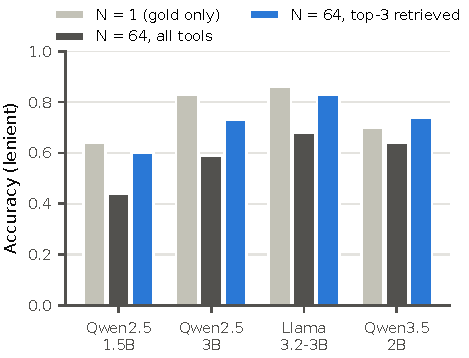
\includegraphics[width=\linewidth]{figures/fig_retrieval.pdf}
    \caption{Lenient accuracy with the gold tool only ($N{=}1$), with all 64 tools, and with the top-3 tools retrieved from the same 64 by Qwen3-Embedding-0.6B (seed-0 catalogs, 100 queries).}
    \label{fig:retrieval}
  \end{minipage}\hfill
  \begin{minipage}[t]{0.49\linewidth}
    \centering
    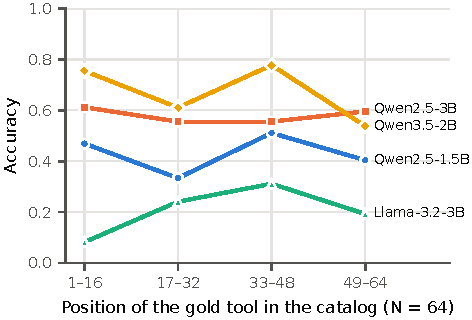
\includegraphics[width=\linewidth]{figures/fig_position.pdf}
    \caption{Accuracy by position of the gold tool in the 64-tool catalog (quartiles). No consistent trend.}
    \label{fig:position}
  \end{minipage}
\end{figure}

\begin{table}[t]
  \centering
  \caption{Retrieval as mitigation (\%). Top-3 tools are retrieved from the same 64-tool catalog (seed 0) and paired per query with the full-catalog run. McNemar $p$ is given for strict / lenient accuracy.}
  \label{tab:retrieval}
  \small
  \begin{tabular}{lccc|ccc|c}
\toprule
 & \multicolumn{3}{c|}{Strict accuracy} & \multicolumn{3}{c|}{Lenient accuracy} & \\
Model & $N{=}1$ & 64 all & 64$\to$top-3 & $N{=}1$ & 64 all & 64$\to$top-3 & McNemar $p$ \\
\midrule
Qwen2.5-1.5B & 64.0 & 44.0 & 60.0 & 64.0 & 44.0 & 60.0 & 0.005 / 0.005 \\
Qwen2.5-3B & 83.0 & 59.0 & 73.0 & 83.0 & 59.0 & 73.0 & 0.013 / 0.013 \\
Llama-3.2-3B & 22.0 & 20.0 & 23.0 & 86.0 & 68.0 & 83.0 & 0.549 / 0.003 \\
Qwen3.5-2B & 70.0 & 64.0 & 74.0 & 70.0 & 64.0 & 74.0 & 0.021 / 0.021 \\
\bottomrule
\end{tabular}
\end{table}

\paragraph{Retrieval itself is nearly solved here.}
Before involving the LLM, we measured how often the embedding model ranks the gold tool among a catalog's top-$k$. On the 64-tool BFCL catalogs, Qwen3-Embedding-0.6B places it first for \RecallQwenNSixtyFourKOne\% of queries and in the top 3 for \RecallQwenNSixtyFourKThree\%. BGE-M3 is somewhat weaker (\RecallBgeNSixtyFourKOne\% and \RecallBgeNSixtyFourKThree\%).
BFCL queries are lexically close to their tool descriptions, so this is an easy retrieval setting. On ToolRet's natively large and diverse corpus, the same embedders are far weaker (\cref{sec:native}).

\paragraph{Top-3 retrieval recovers most of the loss.}
Giving the LLM only the 3 retrieved tools instead of all 64 improves every model (\cref{tab:retrieval}, \cref{fig:retrieval}): by \RetGainQwenOneFive{} points for Qwen2.5-1.5B ($p$\,=\,\RetPQwenOneFive), \RetGainQwenThree{} for Qwen2.5-3B ($p$\,=\,\RetPQwenThree), \RetGainQwenThreeFive{} for Qwen3.5-2B ($p$\,=\,\RetPQwenThreeFive), and \RetLenGainLlama{} lenient points for Llama-3.2-3B ($p$\,=\,\RetLenPLlama).
Qwen3.5-2B with retrieval (\RetQwenThreeFive\%) even exceeds its own $N{=}1$ score (\RetOneQwenThreeFive\%), consistent with the ``too few tools'' effect in \cref{sec:rq2}.

\paragraph{Smaller $k$ is better for these models.}
Because the gold tool is retrieved almost always (\cref{tab:kablation}), the remaining gap is caused by the model, not the retriever. Every additional distractor costs accuracy.
For Qwen2.5-3B, accuracy rises monotonically as $k$ shrinks: \KAccQwenThreeKSixtyFour\% (all 64), \KAccQwenThreeKFive\% (top-5), \KAccQwenThreeKThree\% (top-3), \KAccQwenThreeKOne\% (top-1). Top-1 is within noise of its gold-only score of \AccQwenThreeNOne\%.
The other models are flat between $k{=}1$ and $k{=}5$.
For small models in this regime, the practical advice is to \emph{show as few tools as the retriever's recall allows}.
This contrasts with \citet{singla2026agentweave}, where semantic top-8 retrieval did not help a 1.5B model. A larger $k$ and harder distractors are possible explanations.

\begin{table}[t]
  \centering
  \caption{Effect of $k$ (seed-0 catalogs, 100 queries; strict accuracy, \%). $^\dagger$Lenient accuracy for Llama-3.2-3B. The bottom row is the share of queries for which the gold tool is among the tools shown.}
  \label{tab:kablation}
  \small
  \begin{tabular}{lcccc}
\toprule
Model & top-1 & top-3 & top-5 & all 64 \\
\midrule
Qwen2.5-1.5B & 63.0 & 60.0 & 61.0 & 44.0 \\
Qwen2.5-3B & 81.0 & 73.0 & 68.0 & 59.0 \\
Llama-3.2-3B$^\dagger$ & 83.0 & 83.0 & 83.0 & 68.0 \\
Qwen3.5-2B & 71.0 & 74.0 & 72.0 & 64.0 \\
\midrule
Gold tool retrieved & 97.0 & 100.0 & 100.0 & 100.0 \\
\bottomrule
\end{tabular}
\end{table}
